% En esta seccion se presentan los resultados finales de los experimentos (versión final) mediante figuras y capturas de pantalla debidamente tituladas y referenciadas en el cuerpo del reporte. Analiza las ventajas y desventajas de la metodología aplicada.

\section{Resultados}

En la Tabla \ref{tab:resumen} se reúnen las tres primitivas de esta entrega con
las medidas que pide el manual, la llamada con la que se construyen y el costo
que tiene cada una en vértices y en triángulos. Los tres objetos quedan centrados en el origen y se seleccionan en tiempo de ejecución con las teclas
\texttt{1}, \texttt{2} y \texttt{3}.

\begin{table}[H]
\centering
\begin{tabular}{@{}clccc@{}}
\toprule
\textbf{Tecla} & \textbf{Primitiva} & \textbf{Construcción} & \textbf{Vértices} & \textbf{Triángulos} \\
\midrule
\texttt{1} & Plano de $2\times2$ paralelo a $XY$   & \texttt{Plane(2.0f)}      & 4  & 2  \\
\texttt{2} & Cubo de $2\times2\times2$             & \texttt{Cube(2.0f)}       & 8  & 12 \\
\texttt{3} & Círculo de radio 1                    & \texttt{Circle(1.0f, 72)} & 73 & 72 \\
\bottomrule
\end{tabular}
\caption{Resumen de las tres primitivas implementadas, con su costo en vértices y triángulos.}
\label{tab:resumen}
\end{table}

\subsection{Actividad 1: Plano paralelo al plano XY}
La versión final construye el plano con \texttt{Plane(2.0f)}, con lo que sus
cuatro vértices caen en $(\pm1,\pm1,0)$ y la figura mide las $2\times2$ unidades
solicitadas. El resultado se muestra en la Figura \ref{fig:resultado-plano} en
las dos vistas que pide el manual.

\begin{figure}[H]
    \centering
    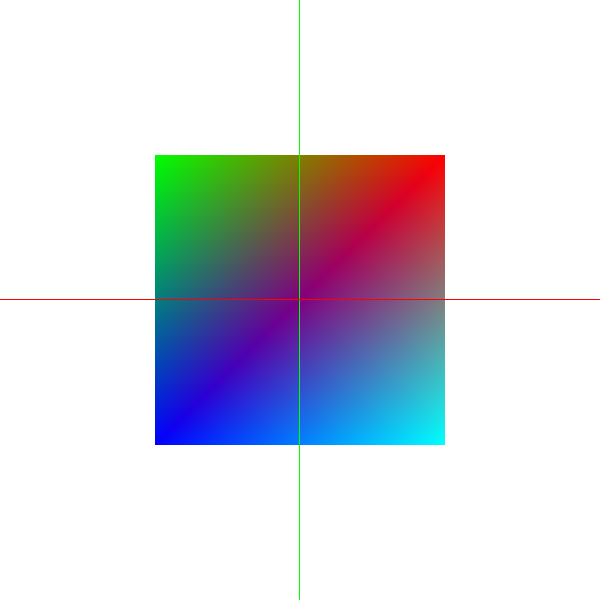
\includegraphics[width=0.45\textwidth]{Imagenes/E1/Plano_Frontal.png}
    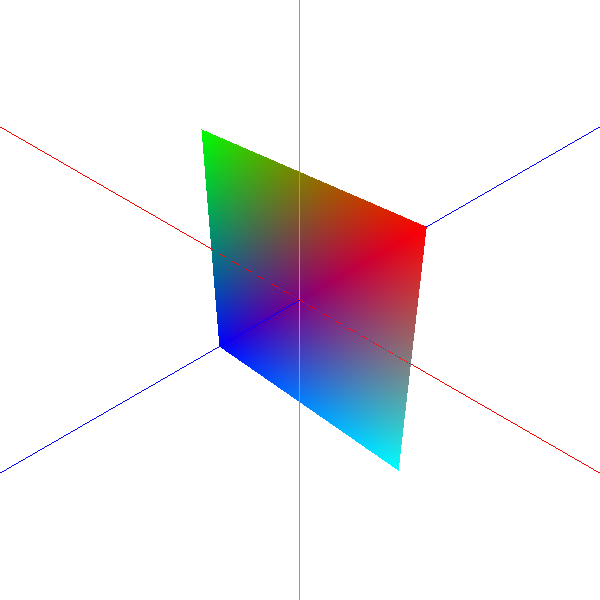
\includegraphics[width=0.45\textwidth]{Imagenes/E1/Plano_Oblicua.png}
    \caption{Resultado final de la Actividad 1: el plano de $2\times2$ unidades centrado en el origen, visto de frente con \texttt{F1} (izquierda) y desde un ángulo oblicuo con \texttt{F2} (derecha).}
    \label{fig:resultado-plano}
\end{figure}

La ventaja de esta solución es que no hizo falta escribir código nuevo: bastó con
leer con cuidado el constructor de la clase que ya venía en el proyecto y elegir
el argumento correcto. Que el constructor reciba el lado completo, y no el
semilado, es además lo que garantiza que la figura quede centrada en el origen
para cualquier tamaño, sin necesidad de aplicar después una traslación con la
matriz de modelo.

Como desventaja, el plano tiene una sola cara en el sentido de que no se le
asignó normal ni se activó el descarte de caras traseras, de modo que se ve
igual por delante que por detrás; eso es suficiente para esta práctica pero
dejará de serlo cuando se agreguen modelos de iluminación. La segunda limitación
es la que apareció en los experimentos: al estar contenido en $z=0$, el plano
comparte profundidad exacta con los ejes coordenados y las líneas de los ejes
quedan por encima de él. Es un artificio del arreglo particular de esta escena y
no un error de la figura, pero conviene tenerlo presente, porque la única forma
de evitarlo sería desplazar ligeramente los ejes o desactivar la escritura de
profundidad al dibujarlos.

\subsection{Actividad 2: Cubo centrado en el origen}
El cubo final se construye con \texttt{Cube(2.0f)}, con los ocho vértices en
$(\pm1,\pm1,\pm1)$ y las seis caras formadas por doce triángulos. La Figura
\ref{fig:resultado-cubo} muestra las dos vistas solicitadas.

\begin{figure}[H]
    \centering
    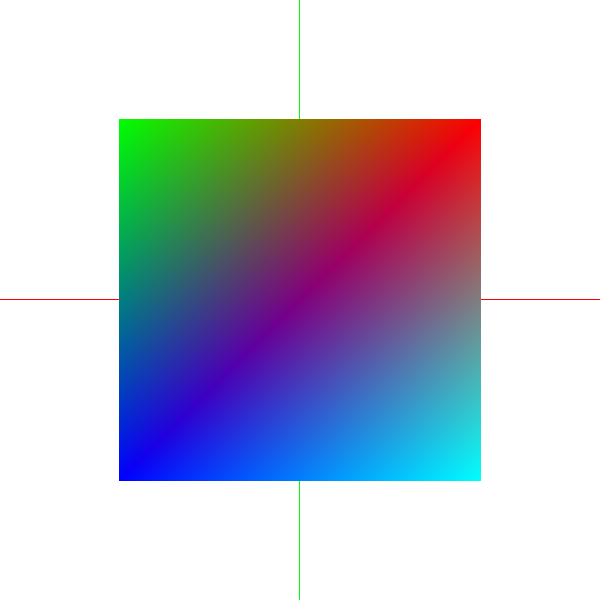
\includegraphics[width=0.45\textwidth]{Imagenes/E2/Cubo_Frontal.png}
    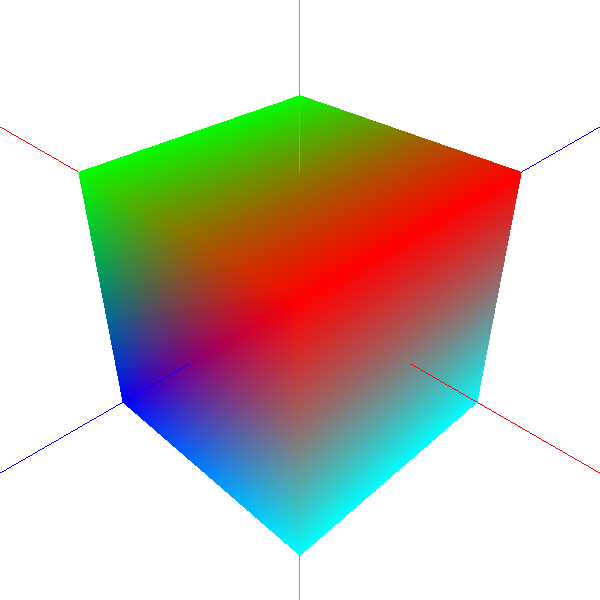
\includegraphics[width=0.45\textwidth]{Imagenes/E2/Cubo_Oblicua.png}
    \caption{Resultado final de la Actividad 2: el cubo de $2\times2\times2$ unidades centrado en el origen, visto de frente con \texttt{F1} (izquierda) y desde un ángulo oblicuo con \texttt{F2} (derecha).}
    \label{fig:resultado-cubo}
\end{figure}

La ventaja principal de la construcción es su economía: ocho vértices bastan
para las seis caras porque cada uno participa en tres de ellas, y esa
reutilización es precisamente lo que permite el arreglo de índices. El degradado
que se observa sobre las caras no costó ningún trabajo adicional; es el
resultado de que cada vértice lleve su propio color y de que la etapa de
rasterización interpole los valores intermedios.

Esa misma economía tiene dos consecuencias que conviene anotar. La primera es
que, al compartirse los vértices, es imposible darle a cada cara un color plano
distinto sin duplicar geometría: habría que pasar de ocho a veinticuatro
vértices, tres copias de cada esquina. La segunda es que el sentido de recorrido
de los índices no es consistente entre las seis caras del proyecto base; mientras
no se active \texttt{glEnable(GL\_CULL\_FACE)} el resultado es idéntico, pero en
cuanto se active, algunas caras desaparecerán y habrá que reordenar los índices.
Lo dejamos así a propósito, porque corregirlo ahora hubiera hecho más difícil
comparar nuestra versión con la del proyecto base, pero queda identificado como
trabajo pendiente.

\subsection{Actividad 3: Círculo de radio unitario}
El círculo final se construye con la clase reescrita, invocada como
\texttt{Circle(1.0f, 72)}. La Figura \ref{fig:resultado-circulo} muestra las dos
vistas, y en la Tabla \ref{tab:circulos} se comparan las dos versiones de la
clase con los números que arrojó la instrumentación del programa.

\begin{figure}[H]
    \centering
    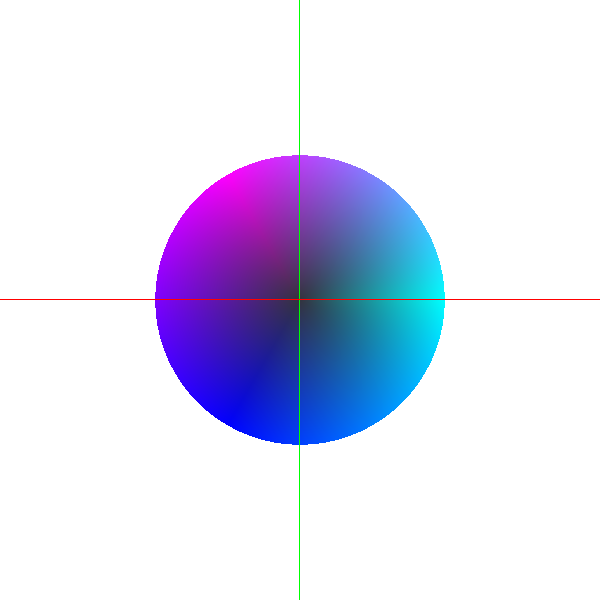
\includegraphics[width=0.45\textwidth]{Imagenes/E3/Circulo_Frontal.png}
    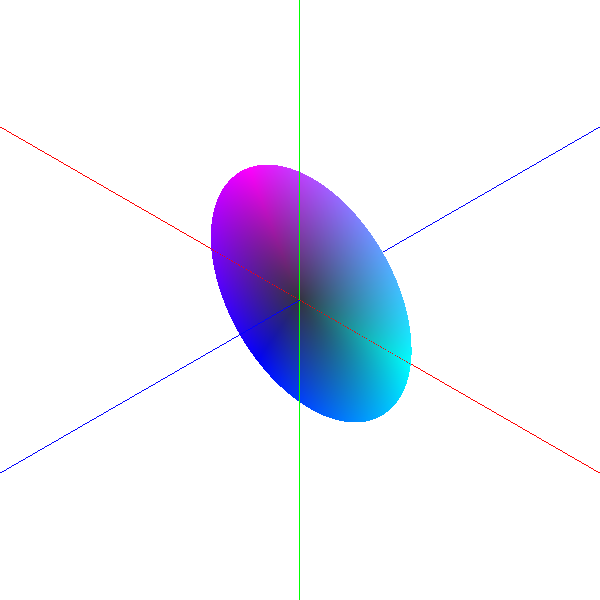
\includegraphics[width=0.45\textwidth]{Imagenes/E3/Circulo_Oblicua.png}
    \caption{Resultado final de la Actividad 3: el círculo de radio unitario centrado en el origen, visto de frente con \texttt{F1} (izquierda) y desde un ángulo oblicuo con \texttt{F2} (derecha), donde se proyecta como una elipse.}
    \label{fig:resultado-circulo}
\end{figure}

\begin{table}[H]
\centering
\begin{tabular}{@{}p{5.6cm}cc@{}}
\toprule
\textbf{Aspecto} & \textbf{Clase del proyecto base} & \textbf{Clase reescrita} \\
\midrule
Vértices generados            & 144            & 73  \\
Índices generados             & 435            & 216 \\
Triángulos con área           & 72             & 72  \\
Triángulos degenerados        & 73             & 0   \\
Índice más grande empleado    & 144            & 72  \\
Índice máximo válido          & 143            & 72  \\
Vértices con color asignado   & 6 de 144       & 73 de 73 \\
Número de lados               & fijo en 72     & parámetro del constructor \\
\bottomrule
\end{tabular}
\caption{Comparación entre la clase \texttt{Circle} del proyecto base y la versión reescrita.}
\label{tab:circulos}
\end{table}

La ventaja de la versión reescrita no es sólo que corrige los dos defectos. Al
volver el número de lados un parámetro del constructor, la figura deja de ser un
objeto fijo y se convierte en una familia de objetos, y esa es justamente la
propiedad que se va a necesitar en las actividades siguientes: la tapa del
cilindro y la base del cono son este mismo círculo con otro radio y otra
posición. Además, el arreglo de índices quedó a la mitad y sin triángulos
degenerados, lo que significa que la mitad del trabajo que hacía la versión
original se gastaba en dibujar triángulos sin área.

La desventaja es que el número de lados quedó fijado en el código en el momento
de la construcción, de modo que cambiarlo obliga a recompilar; para un ejercicio
de esta escala no vale la pena, pero en un programa real convendría reconstruir
la malla en tiempo de ejecución. Una segunda limitación es que la aproximación
poligonal se vuelve visible en cuanto la cámara se acerca lo suficiente: el
número de lados que basta a una distancia deja de bastar a otra, y resolverlo
bien exigiría ajustar la teselación según el tamaño que ocupa la figura en
pantalla, que es un tema que queda fuera del alcance de esta práctica.

\subsection{Sobre la metodología empleada}
Dos decisiones de método resultaron útiles más allá de las actividades
concretas. La primera fue reunir el dibujo de las cuatro mallas en una sola
función en lugar de repetir el bloque de código una vez por figura, como venía
en el proyecto base: además de acortar el archivo, garantiza que las tres
primitivas se dibujen exactamente con la misma cadena de transformaciones, lo
cual es indispensable para que las comparaciones de tamaño entre una y otra
tengan sentido.

La segunda fue agregar el modo de alambre. En las tres actividades hubo al menos
una comprobación que sólo pudo hacerse con esa tecla: contar los dos triángulos
del plano, verificar que al cubo no le faltara ninguna cara y ver el abanico
completo del círculo. En modo relleno, ninguna de esas tres cosas se distingue,
porque la silueta de la figura es la misma esté bien o mal construida por
dentro.

La limitación de la metodología es que todas las verificaciones fueron visuales,
salvo la del conteo de vértices e índices. El caso del índice fuera de rango de
la clase \texttt{Circle} original mostró bien el problema: es un error real que
no produjo ningún efecto en pantalla y que sólo apareció al imprimir los valores
del arreglo. Un método más sólido incluiría comprobaciones automáticas sobre los
arreglos generados, por ejemplo verificar que todos los índices caigan dentro
del rango válido y que ningún triángulo tenga dos vértices repetidos, antes de
enviar la malla a la unidad de procesamiento gráfico.

\subsection{Actividad 4: Cilindro centrado en el origen}

La versión final del cilindro se instanció con los parámetros \texttt{Cylinder(1.0f, 2.0f, 72)}, logrando una geometría sólida, cerrada y centrada en el origen $(0,0,0)$. La estructura final quedó compuesta por un total de 146 vértices (72 por cada anillo perimétrico más 2 vértices centrales para las tapas) y 288 triángulos (144 para el cuerpo lateral y 72 en cada extremo plano). En la Figura~\ref{fig:resultado_cilindro} se aprecian las dos vistas finales.

\begin{figure}[H]
    \centering
    \begin{minipage}{0.48\textwidth}
        \centering
        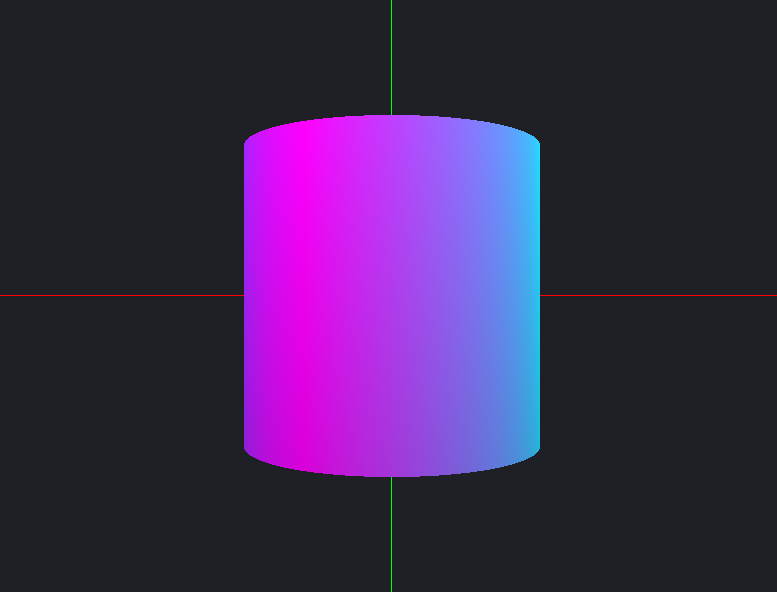
\includegraphics[width=\linewidth]{Imagenes/E4/act4_f1.png}
        \vspace{1mm}
        \centerline{\footnotesize (a) Vista frontal con F1.}
    \end{minipage}\hfill
    \begin{minipage}{0.48\textwidth}
        \centering
        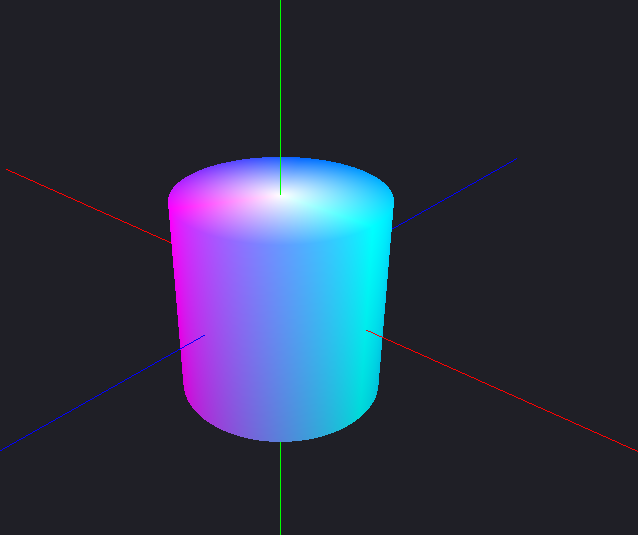
\includegraphics[width=\linewidth]{Imagenes/E4/act4_f2.png}
        \vspace{1mm}
        \centerline{\footnotesize (b) Vista oblicua con F2.}
    \end{minipage}
    \vspace{2mm}
    \caption{Resultado final de la Actividad 4: cilindro de radio 1 y altura 2 centrado en el origen, visto de frente (izquierda) y en perspectiva oblicua (derecha).}
    \label{fig:resultado_cilindro}
\end{figure}

Al ver el cilindro de frente con la tecla F1 (Figura~\ref{fig:resultado_cilindro}a), se ve como un rectángulo de 2 unidades de ancho por 2 de alto, lo que confirma que quedó derecho y bien centrado en el origen porque los ejes pasan justo por en medio. Al cambiar a la vista en diagonal con F2 (Figura~\ref{fig:resultado_cilindro}b), se aprecia claramente su forma redonda y se comprueba que la tapa de arriba quedó bien cerrada.

La ventaja de este método es que poner el cilindro a lo largo del eje Y y usar un solo punto en el centro para tapar las bases hace que la figura quede completa sin gastar memoria de más. Como limitación, dejar el círculo fijo en 72 lados hace que se vea bien y redondito a una distancia normal, pero si acercamos mucho la cámara se alcanzan a notar las líneas rectas de los triángulos.


\subsection{Actividad 5. Esfera centrada en el origen}
La versión final se construye con \texttt{Sphere(1.0f)}, que genera 2592
vértices y, con la triangulación implementada, 5040 triángulos (35 filas de
celdas por 72 columnas, dos triángulos por celda). La Figura \ref{fig:resultado-esfera}
muestra el resultado final en las dos vistas.

\begin{figure}[H]
    \centering
    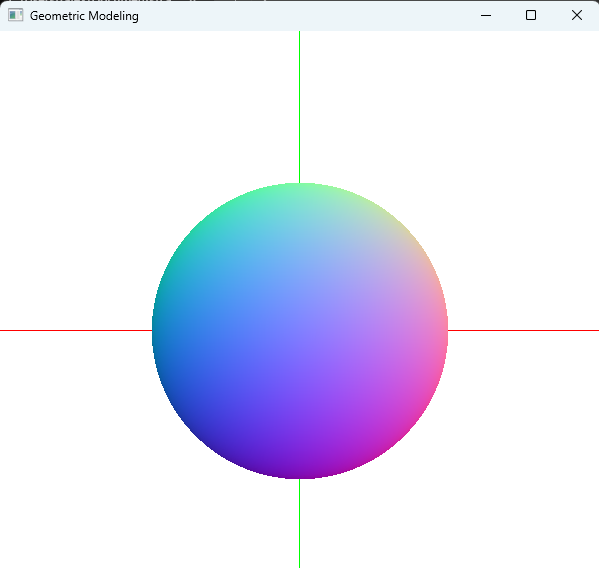
\includegraphics[width=0.45\textwidth]{Imagenes/E5/Esfera_Frontal.png}
    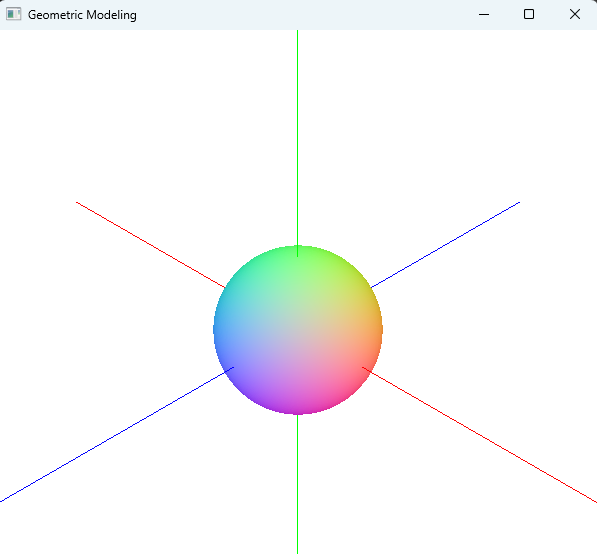
\includegraphics[width=0.45\textwidth]{Imagenes/E5/Esfera_Oblicua.png}
    \caption{Resultado final de la Actividad 5: la esfera de radio unitario centrada en el origen, con el color asignado según la posición normalizada de cada vértice, vista de frente con \texttt{F1} (izquierda) y desde un ángulo oblicuo con \texttt{F2} (derecha).}
    \label{fig:resultado-esfera}
\end{figure}

La ventaja principal de resolver \texttt{buildIndices} por celdas de la
rejilla, en lugar de caso por caso como en el cubo, es que el mismo esquema
--dos filas consecutivas, dos columnas consecutivas, dos triángulos, cerrar
la columna con el operador módulo-- no depende de que la figura sea
específicamente una esfera: cualquier superficie generada por revolución
sobre una rejilla de $\varphi$ y $\theta$ se triangula igual, así que este
mismo código es, en esencia, el que se reutilizará en el cilindro y en el
cono de las actividades 4 y 6, cambiando únicamente la fórmula con la que se
calcula la posición de cada vértice. El color por posición normalizada
también resultó más barato que la interpolación por anclas del círculo,
porque no exige guardar un arreglo de colores de referencia ni calcular en
qué sector cae cada ángulo.

Como desventaja, los ángulos de paso quedaron fijos en $5^\circ$ dentro del
propio método, y no como parámetro del constructor; siguiendo el mismo
criterio que se aplicó al reescribir el círculo, sería preferible exponer el
número de anillos y de columnas como argumentos, de modo que la resolución de
la esfera pueda ajustarse sin recompilar.

\subsection{Actividad 6: Cono centrado en el origen}

Para el resultado final, creamos el cono usando la instrucción \texttt{Cone(1.0f, 2.0f, 72)}, logrando que mida 1 unidad de radio y 2 unidades de alto, quedando justo en medio del origen de coordenadas. En total se usaron 74 puntos (la punta de arriba, 72 puntos alrededor de la orilla y uno más en el centro del círculo de abajo) y 144 triángulos (72 para el cuerpo inclinado y 72 para tapar la base). En la Figura~\ref{fig:resultado_cono} se pueden ver las dos tomas.

\begin{figure}[htbp]
    \centering
    \begin{minipage}{0.48\textwidth}
        \centering
        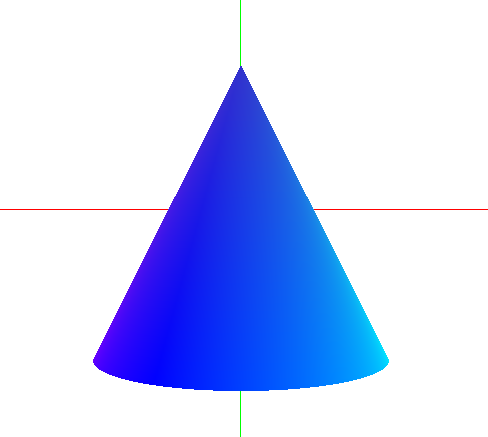
\includegraphics[width=\linewidth]{Imagenes/E6/act6_f1.png}
        \vspace{1mm}
        {\footnotesize (a) Vista de frente (F1).}
    \end{minipage}\hfill
    \begin{minipage}{0.48\textwidth}
        \centering
        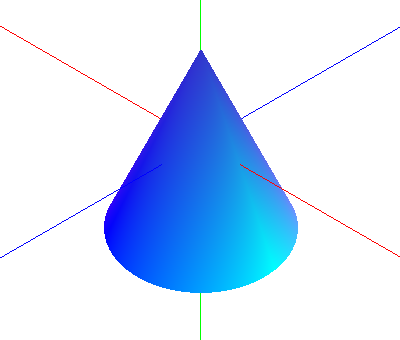
\includegraphics[width=\linewidth]{Imagenes/E6/act6_f2.png}
        \vspace{1mm}
        {\footnotesize (b) Vista en diagonal (F2).}
    \end{minipage}
    \vspace{2mm}
    \caption{Resultado final de la Actividad 6: cono de radio 1 y altura 2 centrado en el origen, visto de frente (izquierda) y de lado (derecha).}
    \label{fig:resultado_cono}
\end{figure}

Al poner la vista de frente con la tecla F1 (Figura~\ref{fig:resultado_cono}a), el cono se ve derechito como un triángulo plano que mide una unidad hacia arriba y una hacia abajo del centro. Cuando cambiamos a la vista en diagonal con F2 (Figura~\ref{fig:resultado_cono}b), ya se nota redondito en 3D y se comprueba que no quedó hueco de abajo.

La ventaja principal de esta forma de trabajar fue que dejamos la figura bien programada desde cero: en vez de dejar valores fijos, le dejamos variables para el radio, la altura y los lados, así que si quisiéramos cambiarle el tamaño a futuro se hace muy fácil. También evitamos que la computadora guardara la punta 72 veces en el mismo lugar, ahorrando memoria y quitando triángulos encimados que no servían de nada. 

Como desventaja, el número de lados se queda fijo en el código; si acercáramos mucho la cámara, la orilla redonda empezaría a verse recta como un polígono y haría falta aumentarle las divisiones. Además, todavía no le calculamos normales a las caras, lo cual ahorita se ve bien con los colores básicos, pero hará falta agregárselo más adelante cuando nos toque poner luces y sombras en la escena.


\subsection{Actividad 7: Escena con OpenGL}

Como resultado se obtuvo una escena con todos los objetos apoyados sobre la superficie, que quedó de color verde con sus colores originales. Del lado derecho se formó una casa con el cilindro naranja barro como base y el cono beige como techo, del lado izquierdo quedaron los cuatro árboles formados por los troncos café claro y los conos verde claro, y al frente las tres esferas alineadas en rojo, amarillo y morado. En la vista oblicua se aprecia la distribución completa de la escena sobre el piso, mientras que en la vista frontal el plano no se alcanza a ver porque la cámara queda a la misma altura que él, y las esferas aparecen encimadas sobre la casa porque están más cerca de la cámara. En la Figura~\ref{fig:resultado_escena} se pueden ver las dos tomas.

\begin{figure}[H]
    \centering
    \begin{minipage}{0.48\textwidth}
        \centering
        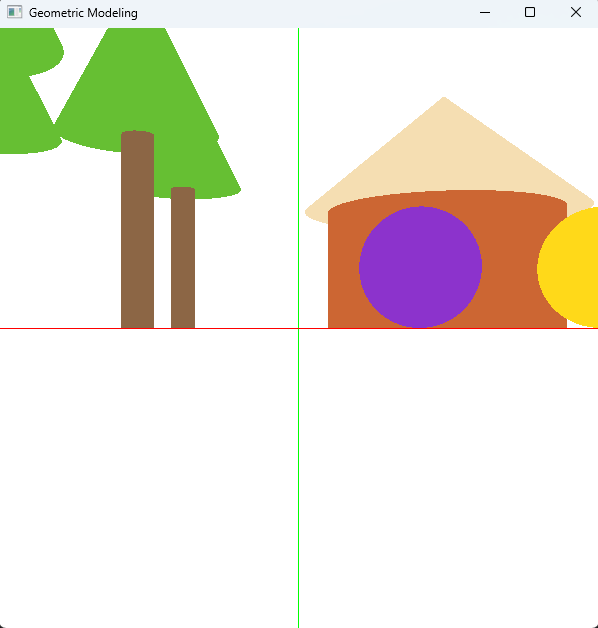
\includegraphics[width=\linewidth]{Imagenes/E7/Escena_Frontal.png}
        \vspace{1mm}
        {\footnotesize (a) Vista de frente (F1).}
    \end{minipage}\hfill
    \begin{minipage}{0.48\textwidth}
        \centering
        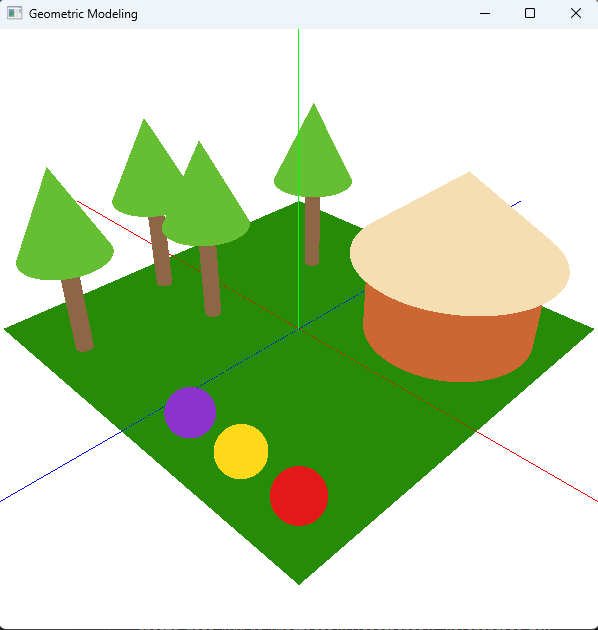
\includegraphics[width=\linewidth]{Imagenes/E7/Escena_oblicua.png}
        \vspace{1mm}
        {\footnotesize (b) Vista oblicua (F2).}
    \end{minipage}
    \vspace{2mm}
    \caption{Resultado final de la Actividad 7: escena construida con el plano, cilindros, esferas y conos, vista de frente (izquierda) y en diagonal (derecha).}
    \label{fig:resultado_escena}
\end{figure}